\section{Source Code as Trees}\label{SourceCodeAsTrees}
The source code of a program is parsed by the compiler, but should also saved in some way so it is possible to manipulate the source code, and performing the phases of the compiler.
This is often done by using a tree, as is it in the \gls{gamble} compiler.

The tree structure is useful for this purpose because every node of the tree can contains information, and have children which then makes it possible to express the productions of a grammar by following a path on the tree from the root to a leaf.
A parse tree separates the source code into different productions of the grammar it represents, but also contains all of the syntax from the grammar, such as parenthesis.
The tree structure also makes it possible to traverse the tree in the same path as the source code is written, which means that the tree is able to express the structure of the source code as well as the statements which are found in the program.
An example of parse tree from the declaration \texttt{int a = 5;} is shown in \myref{image:PST}

\begin{figure}
    \centering
    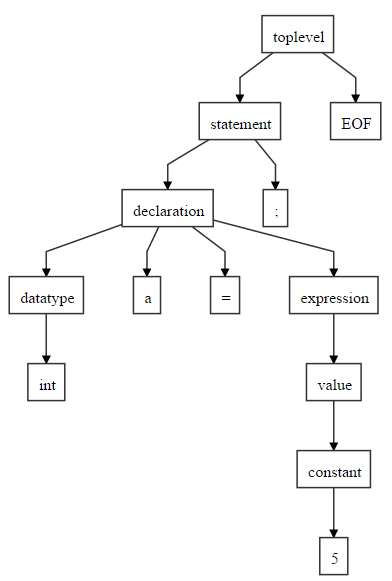
\includegraphics[width=0.5\linewidth]{figures/Trees/PST.PNG}
    \caption{A parse tree from the expression \texttt{int a = 5;} using \glspl{gamble} \acrshort{cfg}.}\label{image:PST}
\end{figure}

The following chapter will explain how the compiler creates a parser to produce these parse trees for the source code, and thus making it possible to use the trees in the compiler.
